\pagebreak

\chapter{Tools zur Unterstützung von CI}
Es gibt eine sehr große Menge an angebotenen Tools am Markt, um CI zu unterstützen. In diesem Kapitel möchte ich vor allem ein paar dieser Tools kurz vorstellen und anhand einiger Merkmale kategorisieren.
\section{Kommerziell vs. Kostenlos}
Grundsätzlich kann man zwischen kostenlosen (meist Open Source) und proprietären, kommerziellen Tools unterscheiden. Es gibt sowohl Gründe für die eine wie auch die andere Art. Ich möchte hier einige Aspekte aufführen, welche eine Toolentscheidung in die eine oder andere Richtung lenken:
\begin{itemize}
	\item \textbf{Technologie}\\
	Zunächst ist zu erwähnen, dass bestimmte Rahmenbedingungen für Unternehmen beziehungsweise Projekte vorgegeben sind. Als Beispiele möchte ich hier bestimmte zu verwendende Technologien erwähnen. Es kann unumgänglich sein ein bestimmtes kommerzielles Produkt zu verwenden, weil nur für diese Technologie zertifizierte Tools erlaubt sind, was meist mit hohem finanziellem Aufwand verbunden ist. Kostenlose Projekte können dies nicht für jede Version leisten und lassen sich deshalb nicht zertifizieren.
	\item \textbf{Usability}\\
	Funktional sind kostenlose Tools meist sehr weit entwickelt. Sie sind nicht selten sogar funktional besser als kommerzielle Tools, weil die Entwicklergemeinde selbst die Funktionalität nach vorne treibt und sogar neueste Entwicklungen einfließen. Ein Manko in vielen dieser Tools ist jedoch die Usability. Nur die größten der kostenlosen Tools schaffen es aufgrund des riesigen Entwicklerhintergrunds, auch die Usability im Auge zu behalten. Ein Beispiel ist Jenkins, bei dem lange Zeit UE/UX das größte Manko war und erst seit Einführung von "`Blue Ocean"' 2016 ist auch der Usability Aspekt in diesem sehr großen Projekt präsent.
	\item \textbf{Regulatorische Einflüsse}\\
	Ein weiterer Aspekt, der Aufmerksamkeit bedarf sind regulatorische Rahmenbedingungen. 
	\item \textbf{Rechtliche Bedingungen}\\
	In der Softwareentwicklung gerade in sehr großen Unternehmen, sind die Kosten für ein System eher zu vernachlässigen. Viel gewichtiger sind rechtliche Absicherungen die man sich durch den Einsatz eines Tools eines finanzkräftigen Unternehmens einkauft. Falls ein Fehler auf einen Bug des CI Systems zurückzuführen ist, und das Unternehmen mit einem prozentualen Anteil des hohen Jahresumsatzes haften muss, so besteht prinzipiell die Chance etwas zurückzuholen. Bei einem kostenlosen Tool existiert dieser finanuzielle Hintergrund nicht. Deshalb ist eine Tendenz zu erkennen, je größer das Unternehmen ist, desto wahrscheinlicher ist der Einsatz eines kommerziellen Tools.
	\end{itemize}
\section{Hosted vs. On-Premise}
Auch dabei, ob man sich selbst um die Infrastruktur des Servers kümmert, oder ein fertiges Produkt mietet, kann man unterscheiden. Dabei gibt es mehrere Aspekte, die beachtet werden müssen, wobei ich einige herausgreifen möchte:
\begin{itemize}
	\item \textbf{Finanzielle Aspekte}\\
	Von finanzieller Seite, muss man klar unterscheiden. Eigene Infrastuktur kostet erstmal Anschaffungskosten, verursacht dann aber auch während des Betriebs laufende Kosten wie Strom, Wartung und Arbeitszeit (was indirekt auch Kosten sind). Auf der anderen Seite bekommt man bei On-Premise Angeboten alles aus einer Hand, trägt kein finanzielles Risiko für Hardwareausfall, und muss dafür einen monatlichen Beitrag zahlen. Für eher kleine Projekte ist es wohl eher von Vorteil On-Premise zu verwenden, in großen Unternehmen und Projekten, wo eine Person sich nur um Build Automatisierung kümmern kann, ist dann wohl eher der eigene Server besser.
	\item \textbf{Nachvollziehbarkeit und Reproduzierbarkeit}\\
	Ein anderer Aspekt ist vor allem für regulatorische Umgebungen wichtig. Hierbei muss es möglich sein, nachzuvollziehen was alles Auswirkungen auf das Ergebnis des Builds hatte. Dazu gehört auch die Build Umgebung selbst. Diese ist jedoch bei vielen On-Premise Angeboten nicht eindeutig zu identifizieren, da diese neue Features einfach live schalten. Auch ist es unmöglich einen Build mit einem bestimmten Stand der Build Automatisierung nochmals laufen zu lassen nach längerer Zeit. Man hat keine Chance, den alten Build Server wiederherzustellen.
	\item \textbf{Datenschutz und Datensicherheit}\\
	Ein nicht zu vernachlässigender Aspekt ist die Sicherheit der Daten und Unternehmensgeheimnisse. Wenn man die Daten aus der Hand gibt, um aus Source Code wirklich ausführbare Programme zu machen, so gibt man auch sein wertvollstes Gut aus der Hand. Man muss dem Unternehmen, das die Services anbietet schon besonders trauen, beziehungsweise sollte es finanzstark sein, um bei Verstößen gegen Schutzbedürfnisse entsprechende Entschädigungen zu zahlen. Die sicherste Methode ist, den Code nicht aus der Hand zu geben und selbst einen Build Server zu hosten. Wenn das nicht möglich ist, sollte auf einen sehr vertrauenswürdigen Partner geachtet werden.
\end{itemize}
\section{Bekannte Vertreter}
Im Folgenden eine kleine Auswahl an Tools, die jedoch keinen Anspruch auf Vollständigkeit erhebt. Ich habe mich auf bekannte Vertreter beschränkt.
\subsection{Jenkins}
Bei Jenkins handelt es sich um ein OpenSource Produkt. Es wurde 2004 gestartet, war zwischenzeitlich im Besitz von Oracle unter dem Namen Hudson und wurde dann geforkt\footnote{Forken ist eine besondere Art des Abspaltens von Entwicklungszweigen, bei dem ein Projekt in mehreren Folgeprojekten resultiert} unter dem Namen Jenkins, unter dem es heute bekannt ist. 
%Es hat eine sehr breite User Basis und auch sehr viele Unterstützer, die Änderungen beitragen. Auch die Menge an Dokumentation ist aufgrund der breiten Userbasis sehr gut.
\begin{center}
  \begin{tabularx}{\textwidth}{lX}
    \toprule
    Kategorie & Wert \\
    \midrule
    Firma & "`The Jenkins Project"'. Dies ist eine rechtliche Dachorganisation und hält die Marke "`Jenkins"' \\
		\addlinespace
    Kosten & Es ist ein Open Source Projekt. Es fallen keine Kosten für die Software selbst an. Nur die Server auf denen Jenkins betrieben wird müssen bei manchen Angeboten (z.B. Cloud) bezahlt werden. \\
		\addlinespace
		Version & 2.121.1 (LTS) , 2.129 (Weekly) \\
		\addlinespace
		SCM Systeme & GIT, TFVC, PVCS, Mercurial, Subversion,...\\
		\addlinespace
		Erweiterbar & Ja, via Plugin System\\
    \bottomrule
  \end{tabularx}
	\captionof{table}{Jenkins Fakten}
\end{center}
Ein Beispiel für das Userinterface von Jenkins ist in \autoref{fig:Jenkins-sample} zu sehen. 
\begin{figure}[H]
  \centering
  \fbox{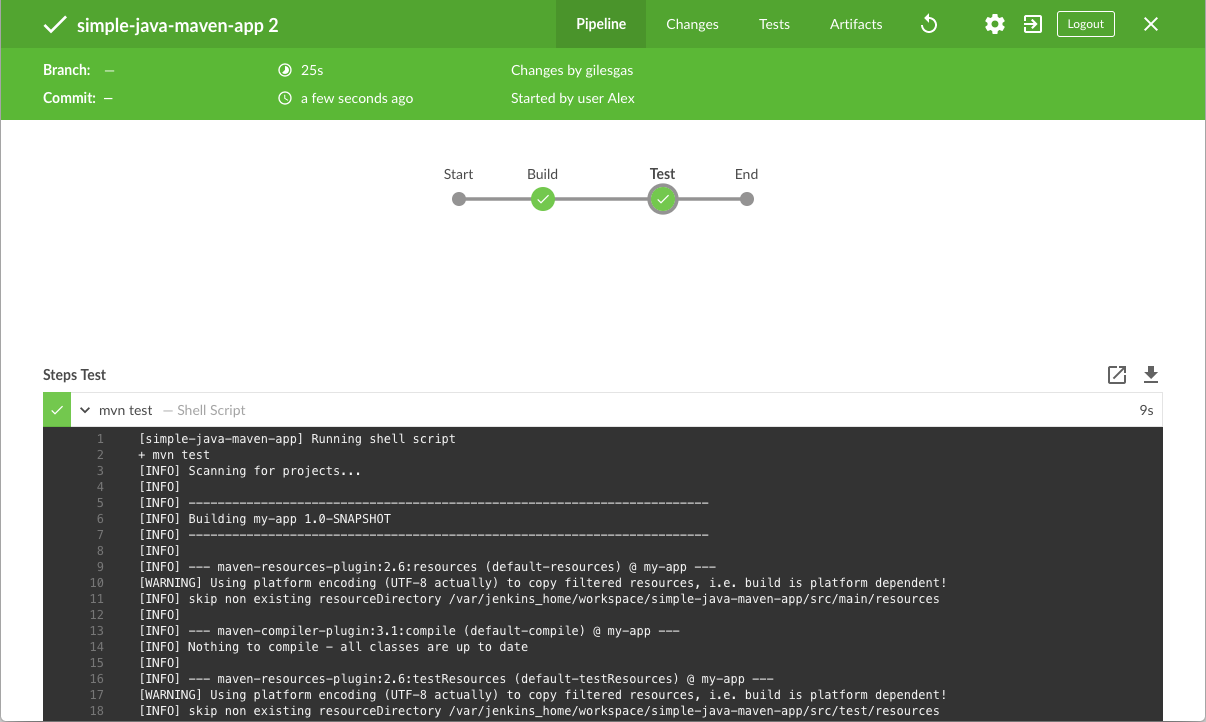
\includegraphics[width=\textwidth]{./Images/Jenkins-sample.png}}
  \caption{Jenkins Weboberfläche \cite{Jenkins-Example}}\label{fig:Jenkins-sample}
\end{figure}
\subsection{TeamCity}
TeamCity ist ein kommerzielles Produkt, das vor allem aus der .NET Welt kommt. Es ist in Java geschrieben und wurde bereits 2006 veröffentlicht. Jetbrains ist eine Firma, die viele Entwicklertools anbietet, um die Produktivität zu erhöhen. 
\begin{center}
  \begin{tabularx}{\textwidth}{lX}
    \toprule
    Kategorie & Wert \\
    \midrule
    Firma &  JetBrains s.r.o., registered seat at Na hřebenech II 1718/10, 14700 Prague 4, Czech Republic \\
		\addlinespace
    Kosten & Teamcity ist ein proprietäres Produkt. Es wird pro Build Agent lizenziert. Der Preis liegt bei etwa 300€ pro Build Agent. Open Source Projekte können das Produkt kostenlos nutzen.\\
		\addlinespace
		Version & 2018.1 \\
		\addlinespace
		SCM Systeme & GIT, TFVC, Mercurial, Subversion,...\\
		\addlinespace
		Erweiterbar & Ja, via Plugin System. Jedoch deutlich weniger Plugins vorhanden als bei Jenkins. Man kann auch selbst Plugins entwickeln.\\
    \bottomrule
  \end{tabularx}
	\captionof{table}{TeamCity Fakten \cite{TeamCity-Marketing}}
\end{center}
Ein Beispiel für das Userinterface von TeamCity ist in \autoref{fig:TC-continuous-integration} zu sehen. 

\begin{figure}[H]
  \centering
  \fbox{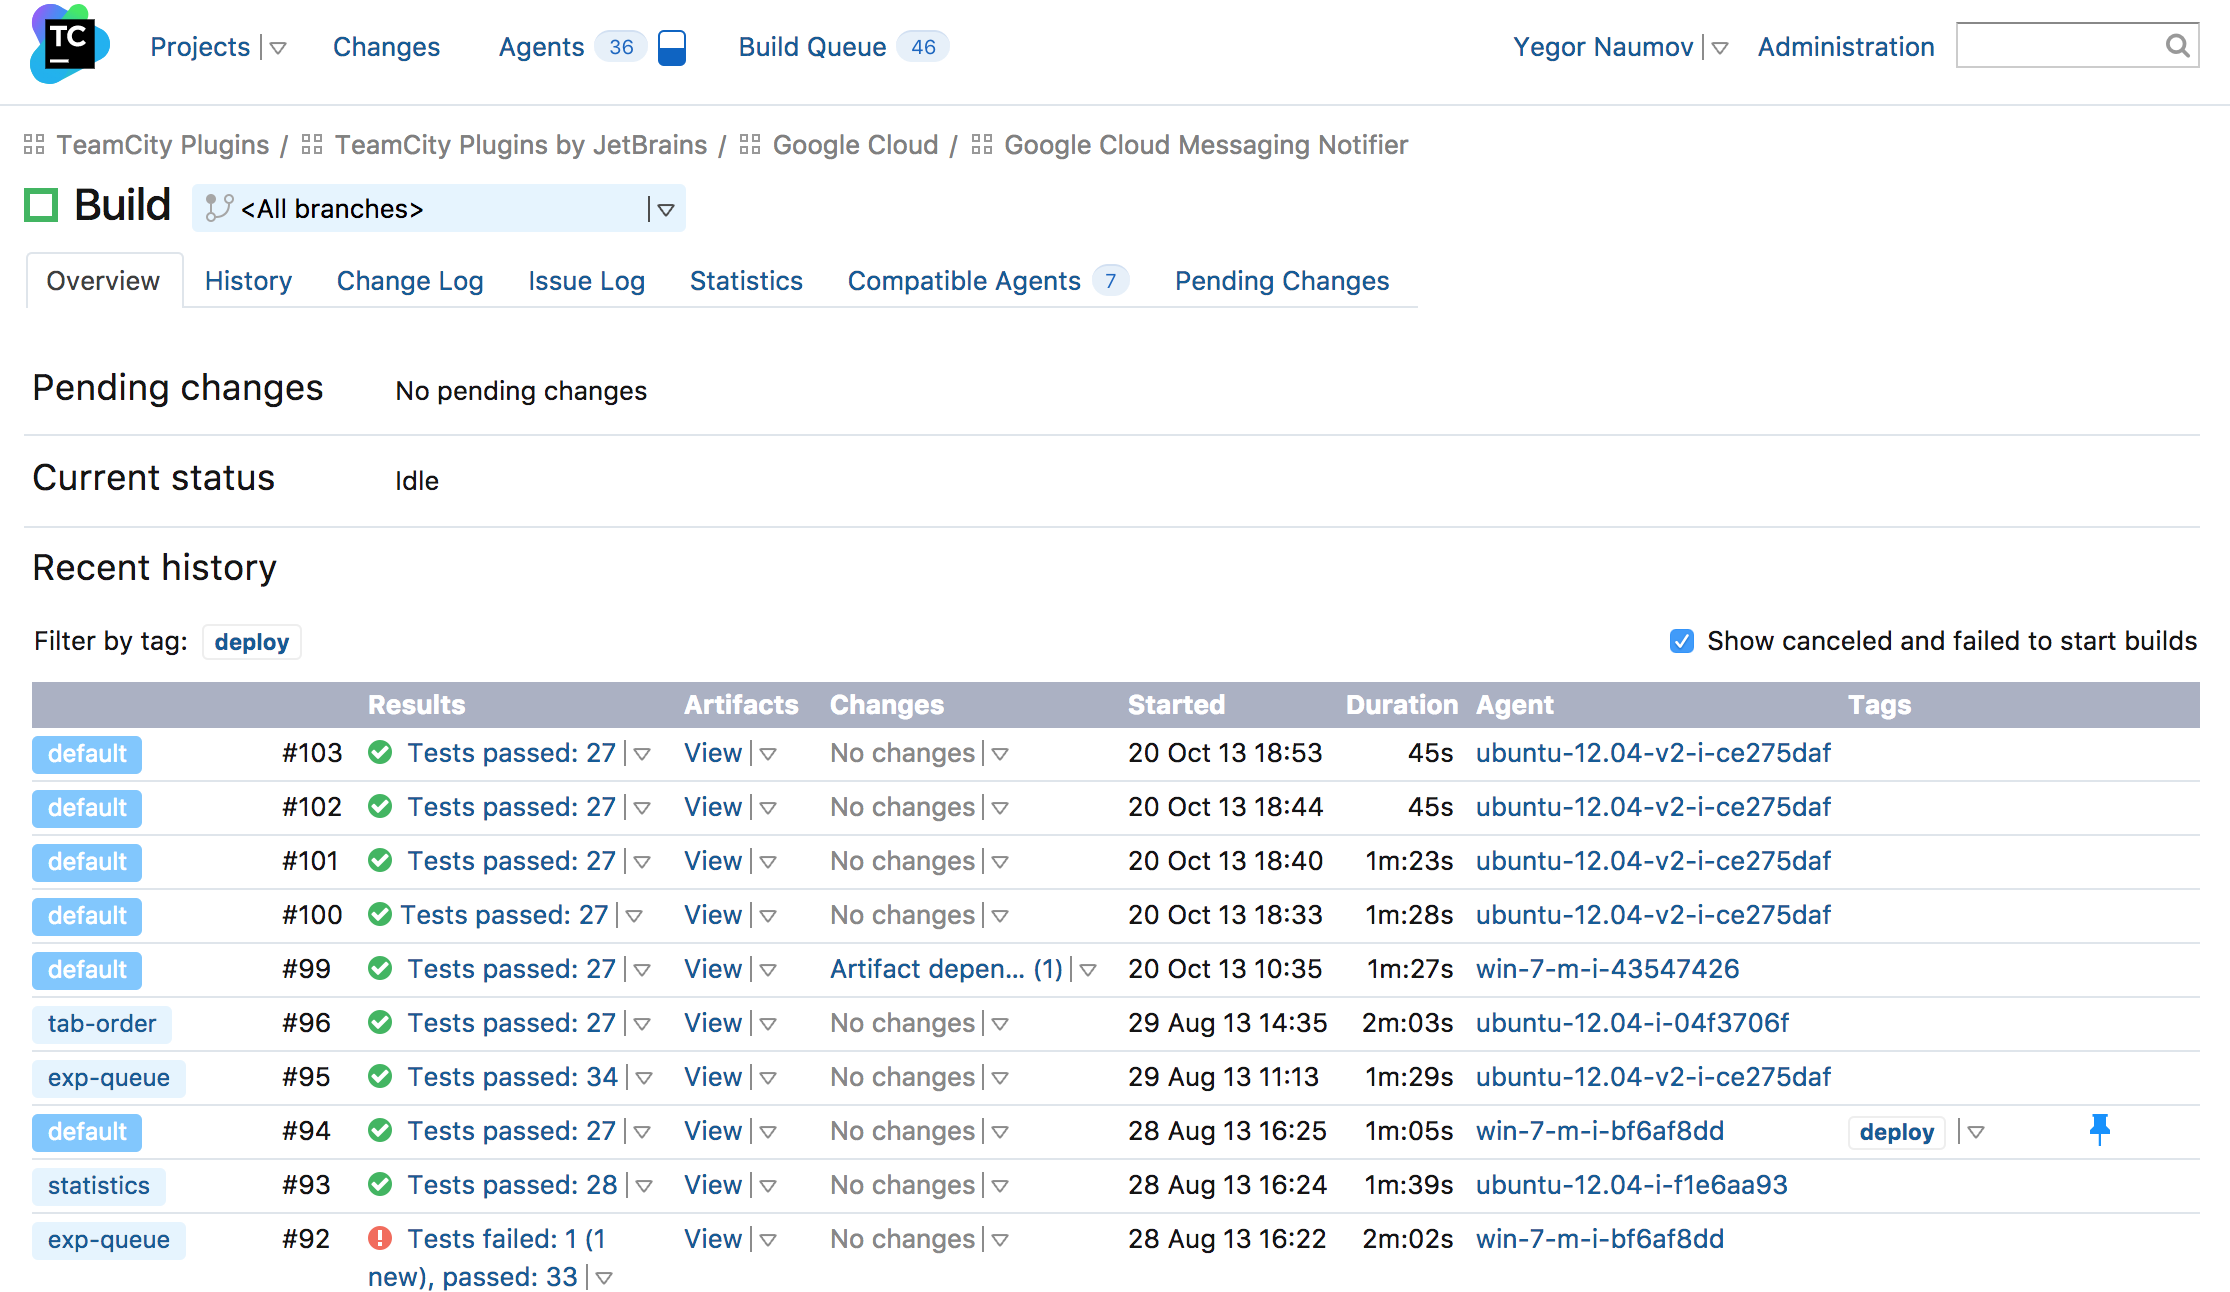
\includegraphics[width=\textwidth]{./Images/TC-continuous-integration.png}}
  \caption{Teamcity Weboberfläche \cite{TeamCity-Marketing}}\label{fig:TC-continuous-integration}
\end{figure}

\subsection{TFS}
Der Teamfoundation Server ist die kommerzielle CI Lösung von Microsoft. Historisch kommt es aus dem .NET Umfeld, entwickelt sich aber in den letzten Jahren immer weiter in Richtung Open Source und CrossPlatform. So ist zum Beispiel die letzte Version der TFS Build Automatisierung lauffähig auf vielen verschiedenen Platformen wie z.B. Windows, Linux, MacOS.\\
Auch sind große Teile der Build Automatisierung OpenSource und auf GitHub verfügbar.
\begin{center}
  \begin{tabularx}{\textwidth}{lX}
    \toprule
    Kategorie & Wert \\
    \midrule
    Firma &  Microsoft \\
		\addlinespace
    Kosten & TFS ist ein kommerzielles Produkt. Es wird pro Nutzer lizenziert, wobei rudimentäre Aufgaben mit der "`Stakeholder Lizenz"' kostenlos sind. Sobald man auch die Build Funktionalität nutzen will, braucht man eine bezahlte Lizenz.\\
		\addlinespace
		Version & 2018 \\
		\addlinespace
		SCM Systeme & GIT, TFVC. Allgemein sehr limitiert, denkbar ist eine manuelle Anbindung, was aber dann von den Tools nicht besonders gut unterstützt wird.\\
		\addlinespace
		Erweiterbar & Ja, an vielen Stellen. Sowohl auf Server- als auch auf Clientseite erweiterbar.\\
    \bottomrule
  \end{tabularx}
	\captionof{table}{TFS Fakten \cite{TFS-Marketing}}
\end{center}
Ein Beispiel für das Userinterface von TFS ist in \autoref{fig:tfs_release_pipeline} zu sehen. 

\begin{figure}[H]
  \centering
  \fbox{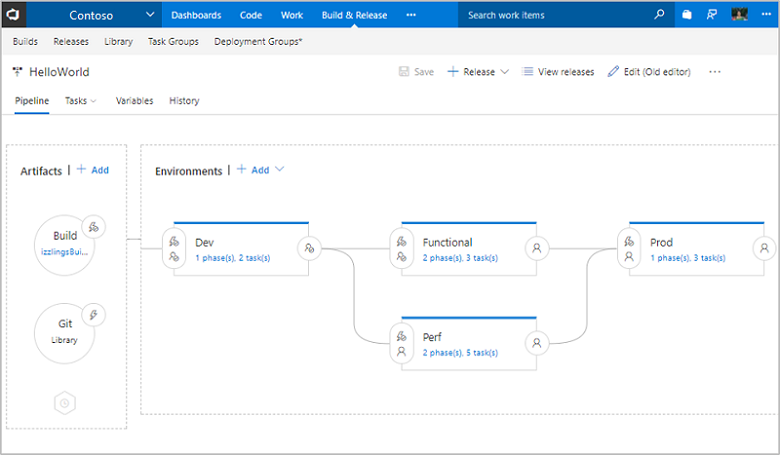
\includegraphics[width=\textwidth]{./Images/tfs_release_pipeline.png}}
  \caption{TFS Weboberfläche \cite{TFS-Marketing}}\label{fig:tfs_release_pipeline}
\end{figure}
\subsection{Travis-CI}
Travis-CI ist ein reiner On-Premise OnlineService. Er erlaubt es automatisch mit jedem GitHib push einen Build zu starten und zu testen.
\begin{center}
  \begin{tabularx}{\textwidth}{lX}
    \toprule
    Kategorie & Wert \\
    \midrule
    Firma &  TRAVIS CI, GMBH \\
		\addlinespace
    Kosten & Travis-CI ist OpenSource. Es ist kostenlos für OpenSource Projekte. Für alle anderen ist es kostenpflichtig.\\
		\addlinespace
		Version & 2.2.1 \\
		\addlinespace
		SCM Systeme & Nur GitHub\\
		\addlinespace
		Erweiterbar & Man kann per yaml den Build Agent so konfigurieren, dass automatisch Compiler usw. installiert werden, aber direkte Erweiterbarkeit gibt es nicht.\\
    \bottomrule
  \end{tabularx}
	\captionof{table}{TFS Fakten \cite{Travis-docu}}
\end{center}
Ein Beispiel für das Userinterface von Travis ist in \autoref{fig:travis} zu sehen. 

\begin{figure}[H]
  \centering
  \fbox{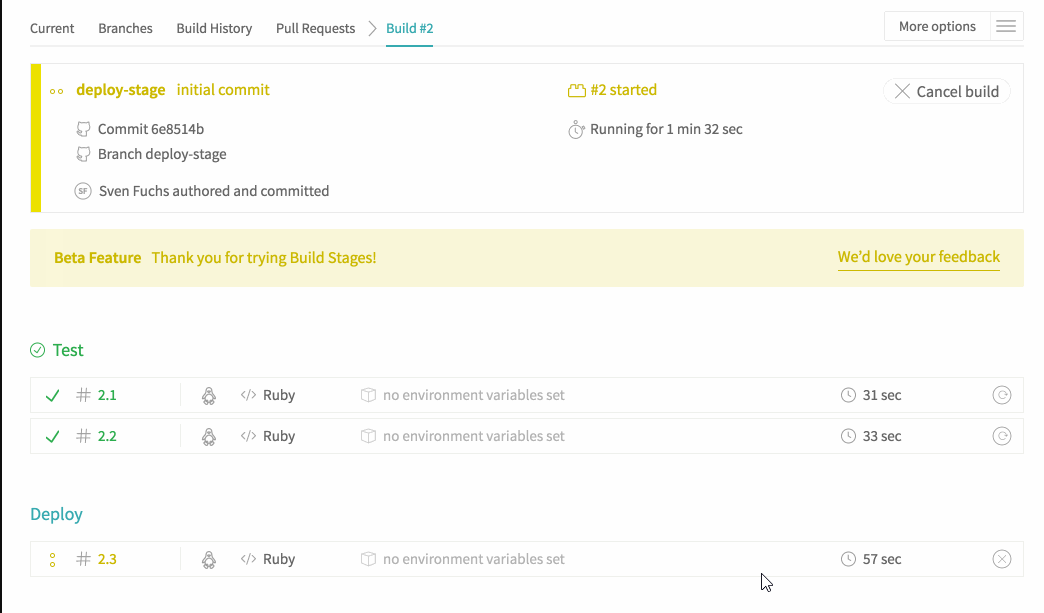
\includegraphics[width=\textwidth]{./Images/travis.png}}
  \caption{Travis Weboberfläche \cite{Travis-build}}\label{fig:travis.png}
\end{figure}